\documentclass{standalone}
\usepackage{standalone}

\begin{document}

\chapter{Methodology}
This chapter describes our process to detect license plate given an input image, and separation of the individual numbers and character sequence from detected license plate. The input image may come from variety of sources. We have put on a validation method to detect if there is actually a license plate in the input image.







\section{Implementation}
We implemented our solution using {\it Python-3.x} using the {\it OpenCV-3} and {\it Tesseract} libraries from Anaconda repository. 
The {\it OpenCV} library provides an extensive collection of image processing functions and techniques which proved very helpful in our implementation. 
{\it Tesseract} is an open source OCR engine made by Google.
Among other libraries, {\it numpy} has been used the most to manipulating 2D arrays.

For testing and analysis we used a separate implementation. In this implementation, we divided entire tasks into sequence of {\bf stages}. This {\it stages} act like individual modules. For example, a stage for Gaussian filter will only apply Gaussian filter to a set of input image and save the output to another folder to make it useful as input for later stages. This approach on testing proved to be quite useful and saved a lot of time during our research.






\section{Overview}
We separate our process into several stages. Each stages contains several steps in it. An overview of all stags in our process is shown in Figure \ref{fig:ProcessOverview}. The process will be described in more details in the following sections.

\begin{figure} 
	\centering
    {\small
      A flow chart will be here containing:\\
      1. Input Image\\
      2. Preprocessing\\
      3. Plate localization\\
      4. Region analysis\\
      5. Plate recognition
    }
	\caption{An overview of the plate detection procedure.} 
	\label{fig:ProcessOverview}
\end{figure}

\begin{description}
\item [Input Image] is a 24-bit colored image with red, green and blue channels.
\item [Preprocessing] stage applies several operations on input image to convert it into an image suitable for feature analysis for later stages.
\item [Plate detection] analyses content of the image to identify and extract the plate like regions.
\item [Region analysis] cleans the extracted plate (removing borders, noise etc), and segments the plate into characters. Also removes bad estimations.
\item [Plate recognition] makes the image ready for {\it Tesseract}.
\end{description}








\section{Preprocessing}
This stage contains a sequence of steps that enhance the plate like regions of an image and output an image that can be used directly for the next stage - plate detection.

\subsection{Rescale}
By minimizing the size of an image we can reduce processing time dramatically. But reducing image may result in loss of information. From reviews, we decided to use the dimension: $640 \times 480$. We re-scale the input image into this dimension at first step. Figure \ref{fig:RescaledSample} shows a sample image.
\begin{figure} 
	\centering
	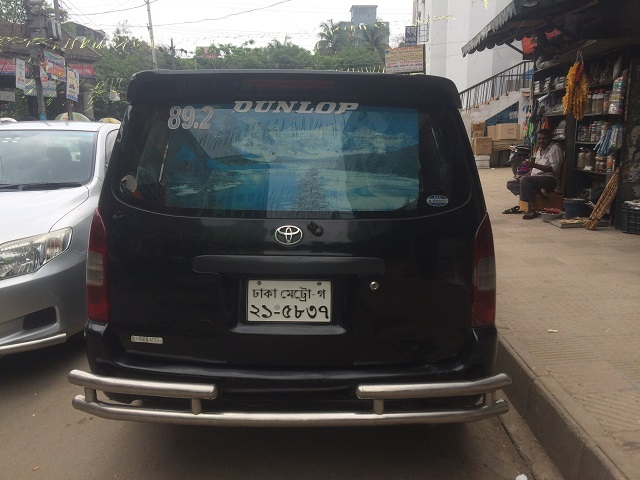
\includegraphics[width=.8\linewidth]{./img/sample/stage0.jpg}
	\caption{A sample input image (rescaled)}
	\label{fig:RescaledSample}
\end{figure}


\subsection{Gray Scale Conversion}
From the 24-bit color value of each pixels $(i, j)$ of the input image, we split the $R$, $G$, $B$ components . Then, 8-bit gray value is calculated using the following formula:
\begin{equation}
gray(i,j) = 0.59 * R(i,j) + 0.30 * G(i,j) + 0.11 * B(i, j)
\end{equation}
\begin{figure}
	\centering
	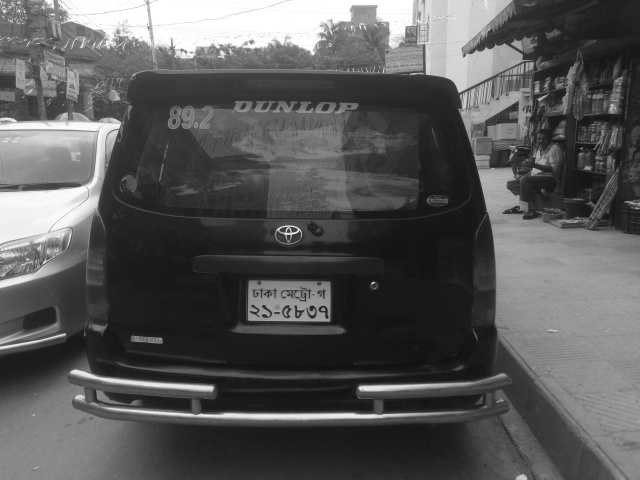
\includegraphics[width=.8\linewidth]{./img/sample/stage1.jpg}
	\caption{A sample gray-scale image} 
	 \label{fig:GraySample}
\end{figure}


\subsection{Vertical Edge Density}
The vertical {\it Sobel operator} (Equation \ref{eq:Sobel}) is used to calculated the edge density. 
\begin{equation} \label{eq:Sobel}
h =
  \begin{bmatrix}
    -1 & 0 & 1\\
    -2 & 0 & 2\\
    -1 & 0 & 1
  \end{bmatrix} 
\end{equation}

Which we could obtain by using $sobel$ function from OpenCV library:
\begin{lstlisting}[language=Python]
sobel = cv2.Sobel(img, cv2.CV_8UC1, 1, 0, ksize=3)
\end{lstlisting}

Next, we applied a low threshold value to the gradient image. In this case, we used an adaptive threshold technique called {\it Otsu’s Binarization} using an offset value of $85$, which we obtained empirically. Result is shown in Figure \ref{fig:SobelSample}
\begin{figure}
	\centering
	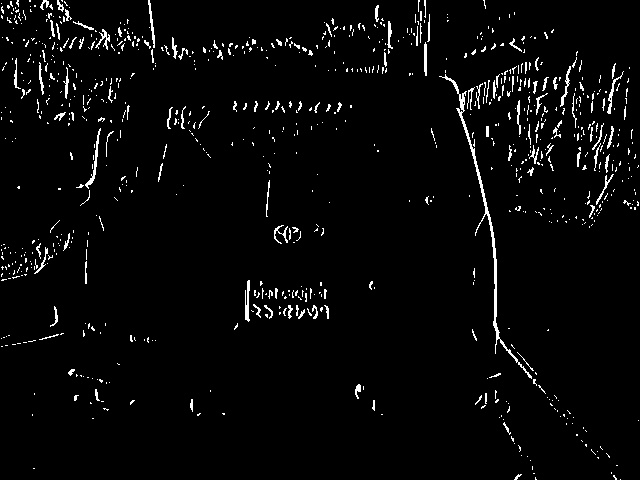
\includegraphics[width=.8\linewidth]{./img/sample/stage2.jpg}
	\caption{After applying Sobel Operator} 
	\label{fig:SobelSample}
\end{figure}

\subsection{Gaussian Filter}
In this step, 2D Gaussian filter is applied to the gradient image from previous step. We used a Gaussian kernel of size $60 \times 60$. To calculate the kernel the formula in Equation \ref{eq:GaussFilter} is used.
\begin{equation} \label{eq:GaussFilter}
g(i, j) = \dfrac{\alpha}{2\pi\sigma^2} \cdot e^{\frac{i^2 + j^2}{2\sigma^2}}
\end{equation}

Here, the blur coefficient $\alpha$ and the $\sigma$ are set empirically. We used $filter2D$ function to apply convolution of on the gradient image
\begin{lstlisting}[language=Python]
gauss = cv2.filter2D(sobel, cv2.CV_64F, kernel)
\end{lstlisting}

As a result we get a nicely blurred image (Figure \ref{fig:GaussianSample}).
\begin{figure} 
	\centering
	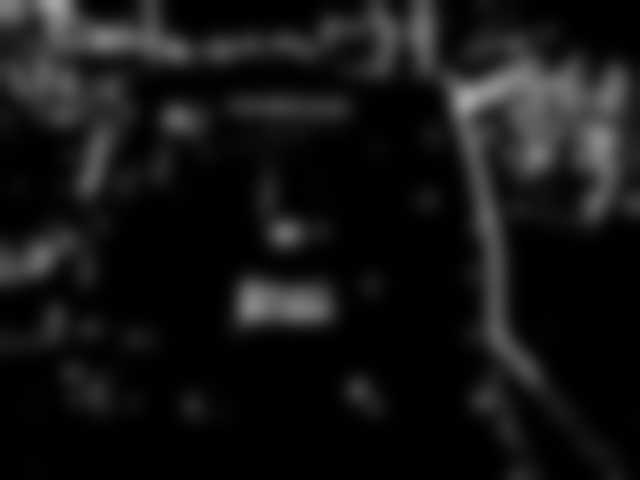
\includegraphics[width=.8\linewidth]{./img/sample/stage3.jpg}
	\caption{Applied the Gaussian Blur} 
	\label{fig:GaussianSample}
\end{figure}

\subsection{Image Enhancement}
We used the Gaussian image to increase the contrast of the image around plate like regions. The formula used is shown in Equation \ref{eq:Enhancement}.
\begin{equation} \label{eq:Enhancement}
I' = f(\rho W_g) (I - \bar{I}) + \bar{I}
\end{equation}
In the equation \ref{eq:Enhancement},\\
$\bar{I}$ = the mean intensity. \\
$I$ = the intensity of the original image. \\
$I'$ = the new enhanced image. \\
$W_g$ = normalized Gaussian image. \\ 
$\rho W$ = the standard deviation of Gaussian image, and \\
$f$ = the weighting function defined in Equation \ref{eq:WeightFunction}.

\begin{equation} \label{eq:WeightFunction}
f(\rho W_g) = 
\begin{cases} 
	\dfrac{3}{ \dfrac{2}{0.3^2} ( \rho W_g - 0.3)^2 + 1 },
    	& \mbox{if } 0 \leq \rho W_g < 0.3  
     \\
    
    \dfrac{3}{ \dfrac{2}{(0.5 - 0.3)^2} ( \rho W_g - 0.3)^2 + 1 },
    	& \mbox{if } 0.3 \leq \rho W_g < 0.5  
     \\
        
    1	& \mbox{if } \rho W_g \geq 0
\end{cases}
\end{equation} 

To increase the efficiency of the calculation the entire image is divided into $8 \times 8$ windows each having the size of $60 \times 80$. For each window we calculated weight and mean intensity using {\it Bilinear interpolation}. Also by using {\it numpy} library for matrix manipulation, we could dramatically decrease processing time.

Figure \ref{fig:EnhanceSample} shows the resultant image. The brightness of license plate area has significantly improved.
\begin{figure} 
	\centering
	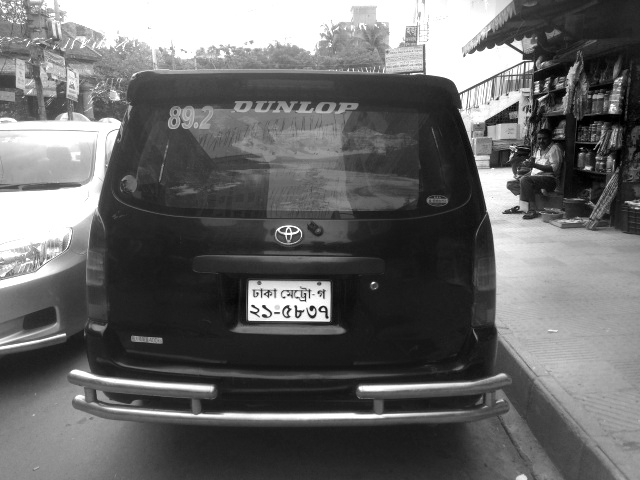
\includegraphics[width=.8\linewidth]{./img/sample/stage4.jpg}
	\caption{Enhanced Image} 
	\label{fig:EnhanceSample}
\end{figure}


\subsection{Matched Filter}
To detect the license plate, next step is to highlight plate like regions from the enhanced image. We used a mixture of Gaussian functions to emphasize the constancy of intensity values within plate-like regions along horizontal direction. Equation \ref{eq:MixtureModel} shows the mathematical model of this function. This function can properly model low edge densities above, below and at the middle of the car plate. 

\begin{equation} \label{eq:MixtureModel}
h(x, y) = 
\begin{cases} 
	A.exp \left(
    	\dfrac{ -\left(x - \dfrac{m}{6} \right)^2 }
        	{ 0.2 \sigma_x^2 } \right),                                      
    	& \mbox{for } 
        	0 \leq x \leq \dfrac{m}{3}, 
            0 \leq y \leq n     
    \\ \vspace{0.2cm}
    B.exp \left( 
    	\dfrac{ -\left(x - 
        			\left( \dfrac{m}{3} + \dfrac{m}{6} \right) 
                \right)^2 }
        	{ 2 \sigma_x^2 } \right),                
        & \mbox{for }
        	\dfrac{m}{3} \leq x \leq 2\dfrac{m}{6}, 
        	0 \leq y \leq n 
    \\ \vspace{0.2cm}
    A.exp \left( 
    	\dfrac{ -\left(x - 
        			\left( 2\dfrac{m}{3} + \dfrac{m}{6} \right) 
                \right)^2 }
        	{ 0.2 \sigma_x^2 } \right),
    	& \mbox{for } 
        	2\dfrac{m}{3} \leq x \leq m, 
            0 \leq y \leq n         
\end{cases}
\end{equation}


In the Equation \ref{eq:MixtureModel}, 
$A$ and $B$ are coefficients of the mixture model. These parameters are set empirically following the condition: $A > 0$ and $B < 0$. 
The symbol $\sigma_x$ is the variance of the main lobe toward x direction. 

This filtering process provides a strong response at plate-like regions (Figure \ref{fig:OriginalMixtureModel}). The result is compared against a predefined threshold value, which is around $80\%$ of the maximum intensity. We call this process as smoothing, and the threshold value as {\it smoothing cutoff}.

\begin{figure}
\begin{subfigure}{.5\textwidth}
  \centering
  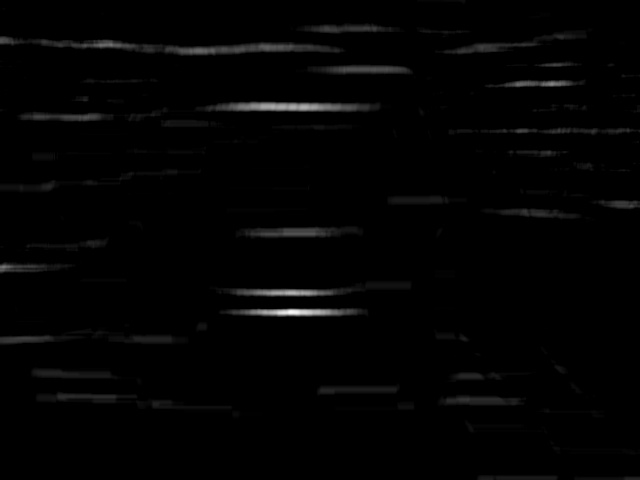
\includegraphics[width=.8\linewidth]{./img/sample/stage5-4.jpg}
  \caption{After applying the mixture model}
  \label{fig:OriginalMixtureModel}
\end{subfigure}
\begin{subfigure}{.5\textwidth}
  \centering
  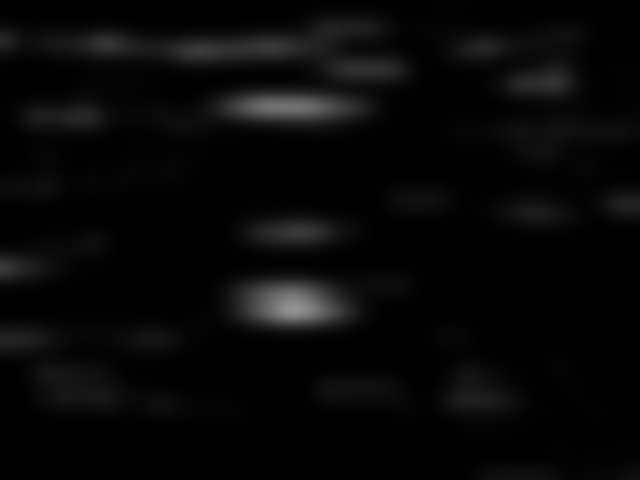
\includegraphics[width=.8\linewidth]{./img/sample/stage5-3.jpg}
  \caption{Gaussian blur on \ref{fig:OriginalMixtureModel}}
  \label{fig:BlurredMixtureModel}
\end{subfigure}
\begin{subfigure}{.5\textwidth}
  \centering
  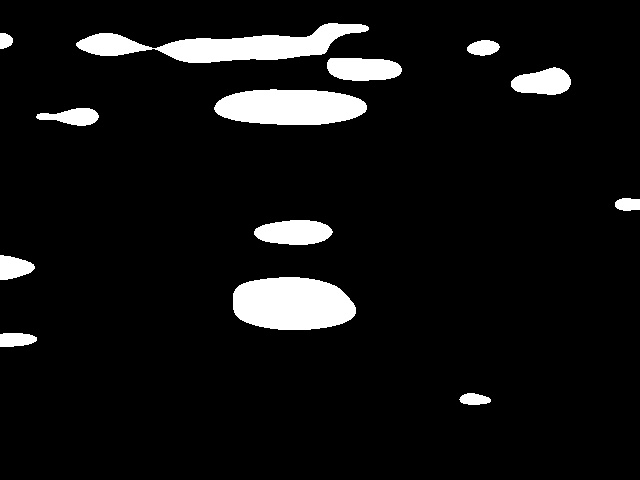
\includegraphics[width=.8\linewidth]{./img/sample/stage5-1.jpg}
  \caption{After applying adaptive threshold}
  \label{fig:ThresholdMixtureModel}
\end{subfigure}
\begin{subfigure}{.5\textwidth}
  \centering
  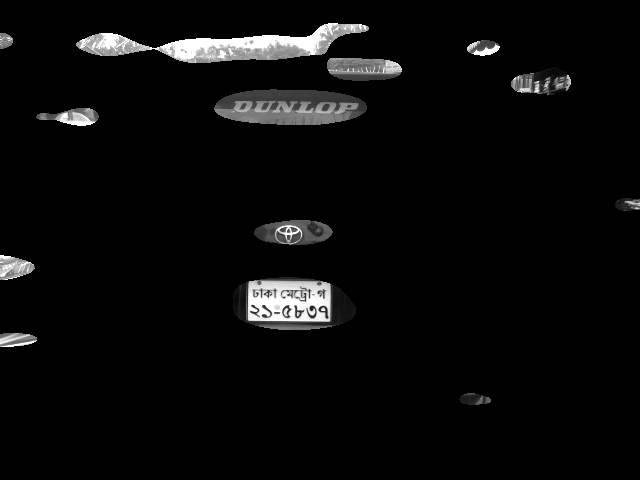
\includegraphics[width=.8\linewidth]{./img/sample/stage5-2.jpg}
  \caption{A see-through view of \ref{fig:ThresholdMixtureModel} with main image}
  \label{fig:GlassViewMixtureModel}
\end{subfigure}
\caption{Images after applying mixture model.}
\label{fig:MixtureModel}
\end{figure}


\subsection{Plate and regions extraction}
This step extracts the license plate and its bounding regions primarily. This does not detect actual license plate. But gives a close approximation to the location of the license plate. First we calculated all contours of the image calculated by mixture model. Next for each contours, we validated the bounding rectangle it is in. If the size of the bounding rectangle is valid, we extract the image of the area and region data. 







\section{Plate Detection}
This section describes the procedure to localize the license plate using the outputs from preprocessing stage. 

\begin{figure} 
	\centering    
	\caption{An overview of the plate detection procedure.} 
	\label{fig:DetectionMethod}
\end{figure}

\subsection{Edge Analysis}
Canny Edge Detection is a popular edge detection algorithm. OpenCV has a direct function to it. We used the default function OpenCV provides to detect all edges of the localized estimated license plate image. 
\begin{lstlisting}[language=Python]
canny = cv2.Canny(img, 100, 200, L2gradient=True)
\end{lstlisting}

\subsection{Contour Analysis}
Canny edge detection works perfectly for most cases and provides an easy to detect contours around plate borders. After passing the canny image to the OpenCV's $findContours$ function, we get a set of contours. For each of these contours several parameters are checked before selecting a contours as a possible plate.

\subsubsection{Width and Height}
The width and height of the detected contour should be above a minimum margin to be recognizable by the OCR. We set the minimum width = $30$ pixels and minimum height = $75$ pixels for estimated plate.

\subsubsection{Area Ratio}
Next we check if the area of the contour is greater than the $10\%$ of the entire image. Remember, we got this image by localizing the plate like regions in pre-processing stage. A possible plate should not have the area below $10\%$ of the entire image.
\begin{equation}
area\_ratio = \dfrac{contour\_area}{image\_area }
\end{equation}

\subsubsection{Aspect Ratio}
Equation \ref{eq:AspectRatio} shows the calculation of aspect ratio of the contour image. From review and observations, we set the minimum value of aspect ratio to $0.3$ and maximum to $0.6$.
\begin{equation} \label{eq:AspectRatio}
aspect\_ratio = \dfrac{contour\_height}{contour\_width}
\end{equation}

\subsubsection{Rotation}
The rotation can be found by the $minAreaRect$ function from OpenCV. 
\begin{lstlisting}[language=Python]
angle = cv2.minAreaRect(cnt)[0]
\end{lstlisting}
If $10 \leq |angle| \leq 80$ we skipped the contour. Because otherwise the contour will be too much skewed to be recognized by any OCR.

\subsection{Extraction}
The region information we get from the previous step is used here to extract the plate image from the original image. We also rotate the image to match with the rotation angle found in previous step. This rotation is done by calculating a rotation matrix of scale $1$ using a OpenCV function:
\begin{lstlisting}[language=Python]
# Calculating rotation matrix M
M = cv2.getRotationMatrix2D(\
		     (center_y, center_x), rotation, 1.0)
\end{lstlisting}

The variable $rotation$ here is calculated from the $minAreaRect$'s $angle$ using Equation \ref{eq:ExtractionAngle}.
\begin{equation} \label{eq:ExtractionAngle}
rotation = 
\begin{cases} 
	-angle, & \mbox{if } angle \leq 45\\
    90 - angle, & \mbox{if } angle > 45
\end{cases}
\end{equation}


\section{Region Analysis}
\subsection{Adaptive thresholding}
\subsection{Geometric rotation}
\subsection{Border removal}
\subsection{More processing}
\subsection{Extract character contours}
\subsection{Reduce bad contours}
\subsection{Validate estimated plate}

\section{Alternative Procedure}
\subsection{Find plate in part of the frame (ROI)}
\subsection{Find the plate using previous locations}

\section{Plate Recognition}
\subsection{Translate coordinates}
\subsection{Extract original plate}
\subsection{Cleaning image}
\subsection{Converting to Binary image}

\section{Character segmentation}
\subsection{Horizontal projection}
\subsection{Vertical projection}


\end{document}